\documentclass[12pt]{article}
\usepackage{geometry} % see geometry.pdf on how to lay out the page. Theres lots.
\geometry{a4paper} % or letter or a5paper or ... etc
% \geometry{landscape} % rotated page geometry

\usepackage{graphicx}
\usepackage[english]{babel}
\usepackage{enumerate}
\usepackage{paralist}
\usepackage{float}
\usepackage{textcomp}
\usepackage{pbox}
\usepackage{tabto}
\usepackage[]{hyperref}
\usepackage{pdfpages}

\newlength{\testlabellength}
\settowidth{\testlabellength}{Test 100.10.10}

%==================================
% Macros.
\newcommand{\qu}{\textquotesingle}
\newcommand{\danne}{\"{o}}

\makeatletter
\newcommand{\setword}[2]{%
  \phantomsection
  #1\def\@currentlabel{\unexpanded{#1}}\label{#2}%
}

\date{} % delete this line to display the current date

%==================================
% Begin document.
\begin{document}

\setlength{\parindent}{0em}
%==================================
% F�rs�ttsblad. 
\begin{titlepage}

\begin{minipage}{0.5\textwidth}
\begin{flushleft} % Responsible persons, write on separate lines
\textit{Lund University\\ ETS170: Requirements Engineering}\\
\end{flushleft}
\end{minipage}
~
\begin{minipage}{0.4\textwidth}
\begin{flushright}

v \ref{ver:latest}

\end{flushright}
\end{minipage}\\[3cm]

	\centering
	{\scshape\LARGE ShopMate \par}
	\vspace{0.5cm}
	\rule{1\textwidth}{.6pt} \par
	{\huge\bfseries Requirements Specification\par}
	\rule{1\textwidth}{.6pt} \par
	\vspace{2cm}
%	{\Large\itshape }

\begin{center}

%==================================
% The version history of this document. 
\textit{\large Version History}

    \begin{tabular}{ | l | l | l | p{5cm} |}
    \hline
    \textbf{Version}	& \textbf{Date}		& \textbf{Description}			\\ \hline
      0.1			& 2015-11-22 			& Release 1			\\ \hline
   	0.2			& 2015-12-7			& Release 2 			\\ \hline
	\setword{1.0}{ver:latest}			& 2015-12-20			& Release 3 			\\ \hline
    \end{tabular}
\end{center}

%==================================
% The authors down to the left. 
\vfill
\begin{flushleft}
	\textit{By Group I:}\\
	Daniel Dornl\danne v\par 
	David Cartbo\par
	Jonathan Lundholm\par 
	Kristoffer Hilmersson\par
	Marcus Hilliges\par 
	Thomas Strahl\par
	\end{flushleft}
\end{titlepage}
\newpage

\tableofcontents

\newpage

%==================================
% Introduction
\section{Introduction}
Our customer is planning to open a brand new shopping mall and would like to stand out from their competitors. In order to do this and at the same time 
increase customer value, they have asked us to develop an application called ShopMate for the mall. The product ShopMate will help the customers of the 
mall, e.g. creating a shopping list, receiving special offers and finding their way around the mall. The shop owners are hoping the product will increase sales 
and attract new customers to the mall. They will also be able to promote their individual stores through the application.

%==================================
% Business Goals
\subsection{Business Goals}

The purpose of the product is to enhance the experience of a customers visit by offering some features that facilitates their stay. 
With the provided functionality of the product, the customer satisfaction will increase, as well as the number of visiting customers and the 
number of sales for the stores. This will enable the mall owner to charge the stores higher rents and a higher revenue for the stores in the mall.

\subsection{Terminology}
	\begin{description}
	\setlength{\itemsep}{0pt}
	\item [The product] is referring to the ordered system. The product consists of an application for the operating systems; Android and iOS. 
	In addition to the application there shall be support for a Smart-watch and a server/database to store information in.
	\item [Smartphone] is a mobile phone with internet connection, touch screen and possibility to install applications from Google play store or App store depending if the Smartphone runs Android or iOS as operating system.
	\item [Smart-watch] is an iOS- or Android-wearable, in other words it\qu s a connected device that communicates with a Smartphone and can run lightweight applications.
	\item[The user] is referring to the person using the application on their device.
	\item[Device] is referring to the unit the user is running the app on, e.g. Smartphone and Smart-watch.
	\item [Offers] are store-products or services that are being sold att a lower price in the stores a the mall. Offers are displayed on the user\qu s screen of their devices.
	\item [The server/database] is where all data about stores, offers, store-products, maps and so on are stored.
	\item [Store] refers to companies located in the mall. 
	\item [Store-product] refers to items/products being sold in the stores, not the product that is being developed.
	\item [Location] refers to the location of a user or a store in the shopping mall. 
	\item [Shopping list] refers to a list with items or store-products that the user has added to a list and intends to buy while at the mall.
\end{description}

The requirement ID\qu s are meant to help the reader to know what section of the report they address. 
They also increase awareness in the project and can be used to not have to state the whole requirement every time they are mentioned. \\�\par

The requirement ID\qu s are formatted after which category they are active within, and complemented with a few words describing what function they fulfill. For example a business requirement starts with "Business" followed by their function, e.g. "Customer satisfaction". Which will give the following requirement ID: \textit{Business --- Customer satisfaction.} The same technique is used for all the other areas of the requirement specification as well. 

%==================================
% This is where the requirements start.
%==================================


%==================================
% Business
\section{Business}

Here we address requirements regarding the business goals for the product. 
This is how our customer will be able to profit from the product. \\�\par

\underline{Business --- Customer satisfaction} \\ The product shall increase the shopping malls customer satisfaction.\\ \par

\underline{Business --- Mall revenue} \\ The product shall increase the malls yearly revenue by 4�\%. \\ \par

\underline{Business --- More customers} \\ The product shall help increase the number of visiting customers to the mall by  \\ 8 \%.\\ \par

\underline{Business --- Increased sales} \\ The product shall help increase the number of sales the stores have by 3 \%. \\ \par

\underline{Business --- Impulse sales} \\ The product shall increase the number of impulse buys of store-products by 10 \%.

%==================================
% Context Diagram

\section{Domain Overview}

\subsection{Context Diagram}
ShopMate has an excessive inner domain, communicating with various other systems. In order to fulfill some of the fundamental requirements, 
this is necessary. Figure \ref{fig:contextdiagram} below represents the domain level of ShopMate, displaying the systems needed to provide the desired functionality.  \\�\par

We are only implementing the ShopMate application, and thus only communicating with the other (already existing) systems interfaces 
(Parking System, Navigation System, Public Transportation, database). A minimalistic version of the product is also to be implemented on 
Smart-watches, where only the essential parts of the application is used. For more information about what functionality exists on what 
device and what functionality is limited by not having internet connection see table 1 and 2 in the appendix on page \pageref{app:A}. 
The following states the overall requirement defined by the context diagram. \\�\par

\underline{Context diagram --- Functionality} \\  The product shall support the interactions defined in the context diagram.\\ \par

\underline{Context diagram --- Interface} \\ The product shall support communication with the existing interfaces that are present in the mall today.

\begin{figure}[H]
    \centering
    \includegraphics[width=0.95\textwidth]{../files/Context_Diagram.png}
    \caption{The context diagram for the ShopMate system, describing its domain level.}
    \label{fig:contextdiagram}
\end{figure}

The Location System is used to locate where the user is in the mall to make navigation possible. Mall Data System is a database that contains all the necessary 
data concerning the stores, products, offers, prices and stock balance. Public Transport refers to the system used to be able to provide the users with timetables 
of the local public transport. Parking System is the external system used by ShopMate to find parking spots and finding parked vehicles.

%==================================
% Navigation

\section{Navigation}
Navigation address requirements that involve locating the user, stores and other important 
resources in the product which could mean the GPS or maps.  \\�\par

 \underline{Navigation --- Scenario} \\ 
 The app shall support the following scenario: \\�\par
 
 \textit{"Jonathan decides to go to his local shopping mall to try out their new app: ShopMate. He has a good idea of what he wants, 
 so he creates a shopping list of the products that he wants. Now, Jonathan wants to follow the resulting route generated  by ShopMate. 
 Halfway to the first store, he needs to go to the bathroom and wants to use the public information provided by the app. Based on his current position, ShopMate displays the nearest restroom."} \\�\par

 \underline{Navigation --- Find store} \\ The product shall assist the user to navigate to a store in the mall. \\�\par
 
  \underline{Navigation --- Find public info} \\ The product shall assist the user to navigate to public information as listed above. \\�\par

\underline{Navigation --- Find location} \\ The product shall be able to assist the user to get from its current location to a specified 
location by the user in the mall. e.g. a store, toilet, elevator and so on. \\ \par

 \underline{Navigation --- Guide to specific location} \\ The product shall have a function for directing the user to a specific location in the mall. \\�\par

\underline{Navigation --- Public information} \\ The product shall provide public information, such as location of handicap toilets, 
elevators, ATM machines, etc. With this information the user shall be able to navigate to the correct position in the mall. \\�\par

 \underline{Navigation --- Precision of positioning} \\ The product positioning shall have a resolution no greater than 5 m. 
 
   \begin{figure}[H]
    \centering
    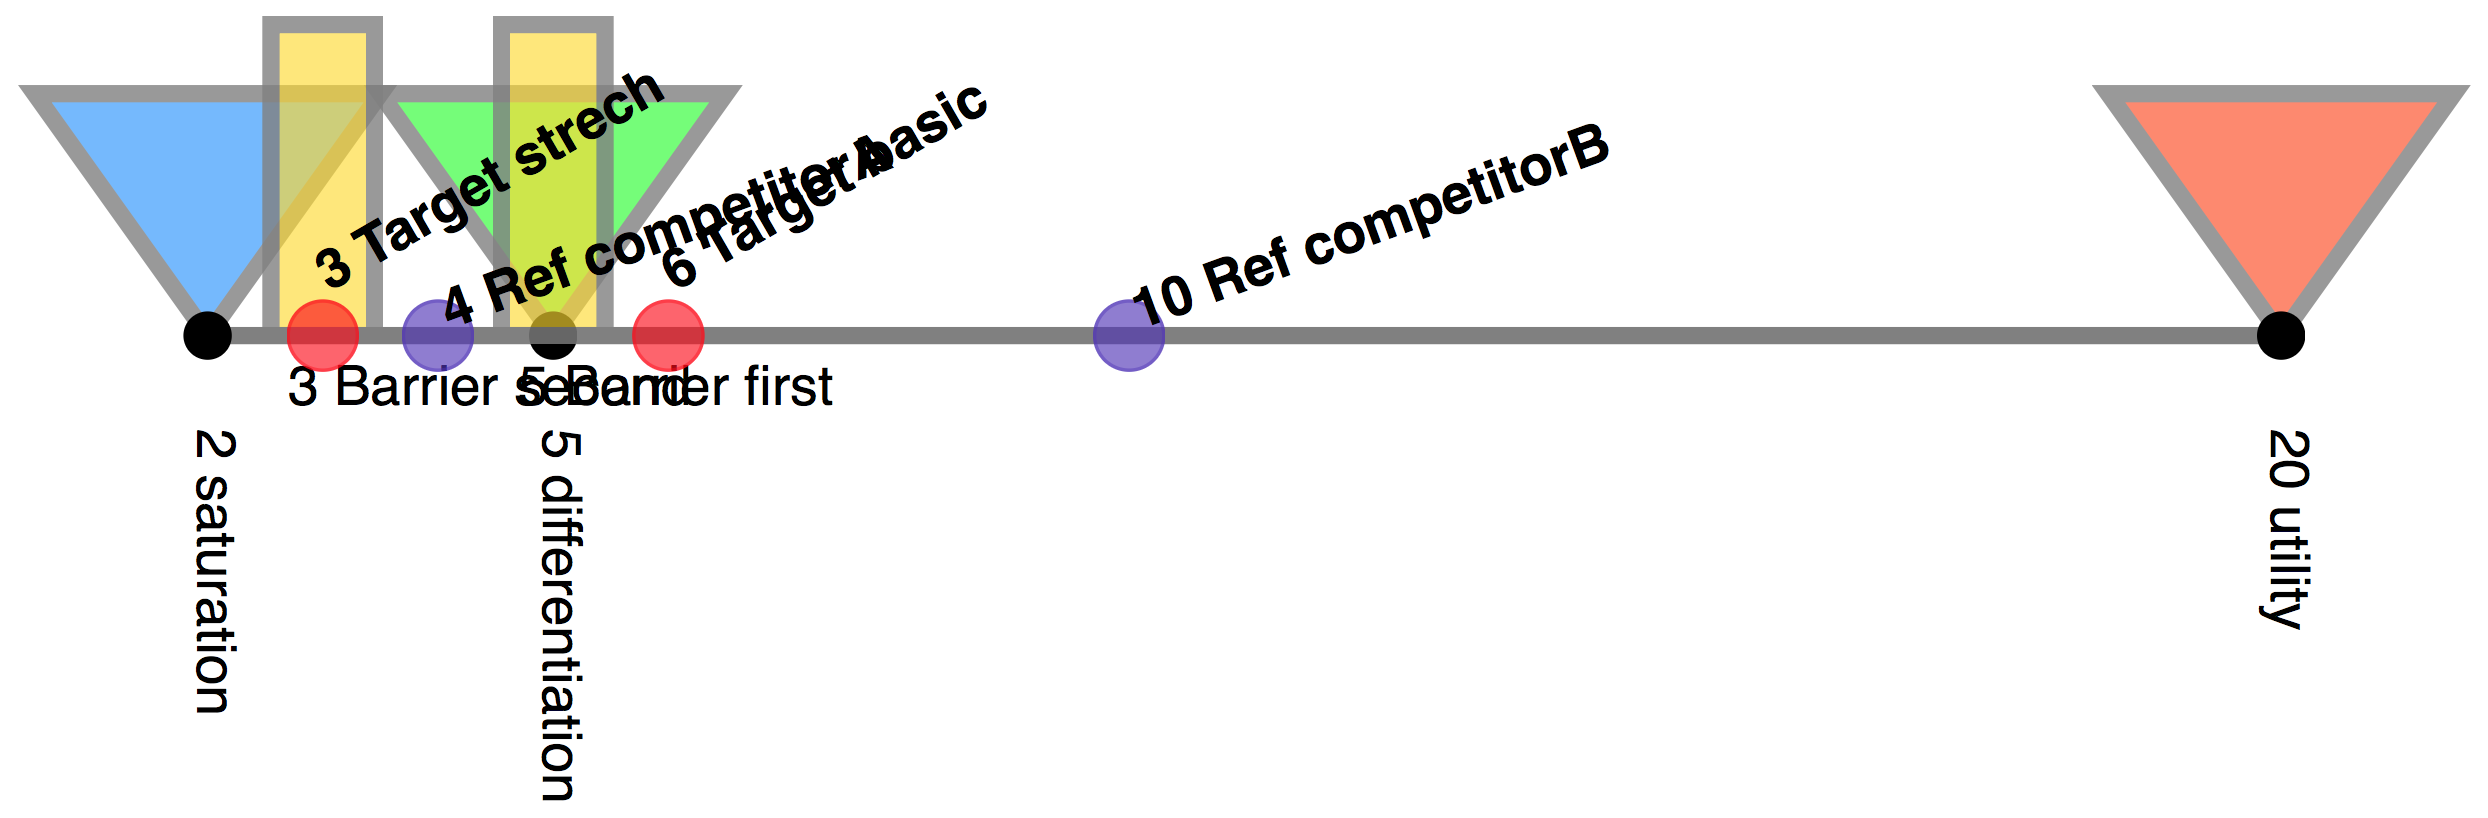
\includegraphics[width=0.9\textwidth]{../files/parkingquper.png}
    \caption{\textit{Navigation --- Precision of positioning} was elicitied using the QUPER shown in the figure.}
    \label{fig:parkquper}
\end{figure}

 \underline{Navigation --- Locate speed} \\ The product shall locate the user within 5 seconds after starting the app 90 \% of the time. 
 
 \begin{figure}[H]
    \centering
    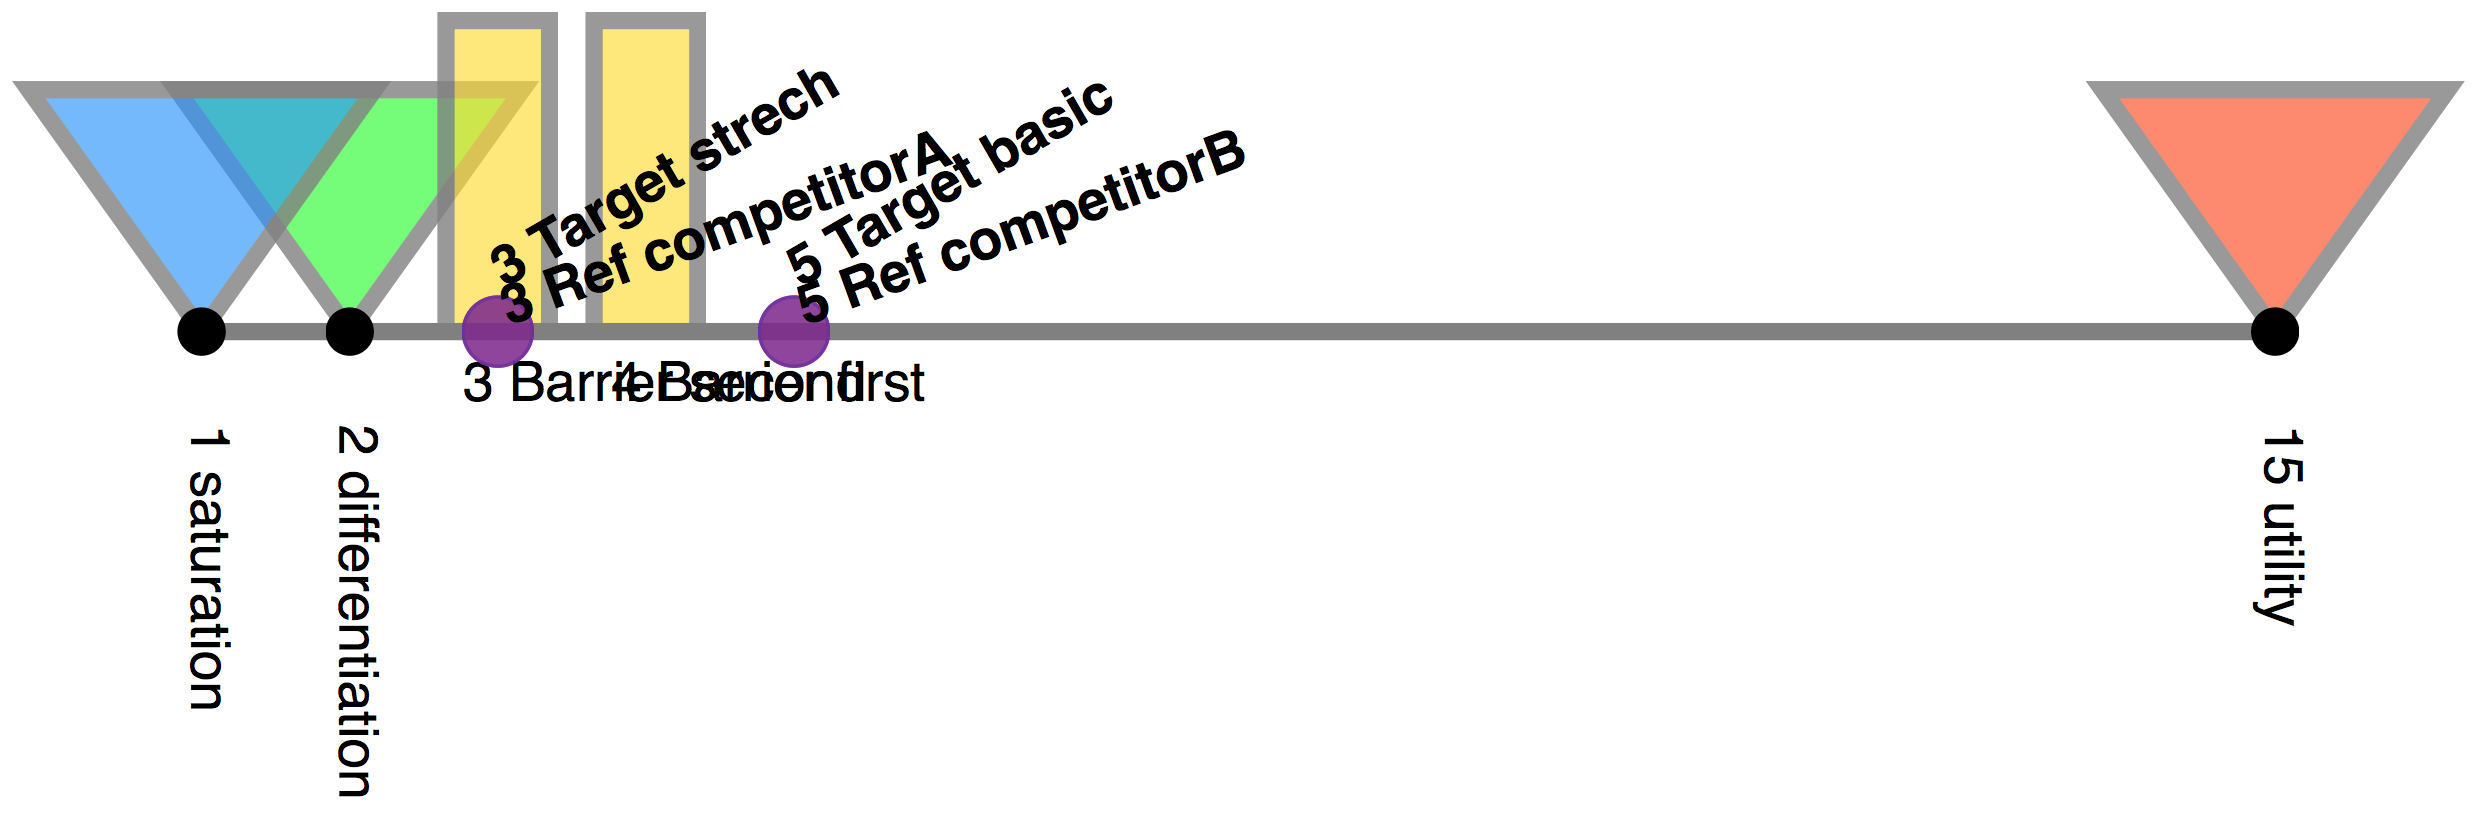
\includegraphics[width=0.9\textwidth]{../files/navquper.png}
    \caption{\textit{Navigation --- Locate speed} was elicitied using the QUPER shown in the figure.}
    \label{fig:navquper}
\end{figure}

 \underline{Navigation --- API} \\ The product shall use Google API for locating the user. \\�\par
 
 \underline{Navigation --- Find user in mall} \\ The product shall have a function for locating the user in the shopping mall. This function 
will help the user to know what floor he or she is on, and where on that floor the user is currently located. See figure \ref{fig:nav} for more information. \\ \par

%==================================
% Data

\section{Data}
This section describes how data is to be stored, and how to get information 
(e.g. readable to humans) out of stored data. There are references to figures 
that illustrate how some of the data is to be stored. \\�\par

  \underline{Data --- Store products} \\ The database shall provide information on what products stores sell.�\\�\par
  
   \underline{Data --- Product information} \\ The product shall have data provided by the stores on stock balance, prices and offers on store-products.\\ \par


 \underline{Data --- Products} \\ The database shall contain the store-products sold in the shopping mall. \\�\par
 
   \underline{Data --- General store information} \\ The product shall have a database to store general information about the stores. \\�\par

 \underline{Data --- User attributes} \\ The product shall store data according to figure \ref{fig:user}.  

\begin{figure}[H]
    \centering
    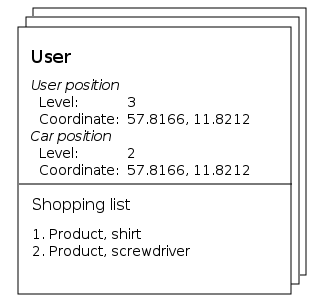
\includegraphics[width=0.4\textwidth]{../files/vw_user.png}
    \caption{Refers to the requirement \textit{Data --- User attributes.}}
    \label{fig:user}
\end{figure}
 
\underline{Data --- Data relationships} \\ The product shall store data according to figure \ref{fig:er}. 

   \begin{figure}[H]
    \centering
    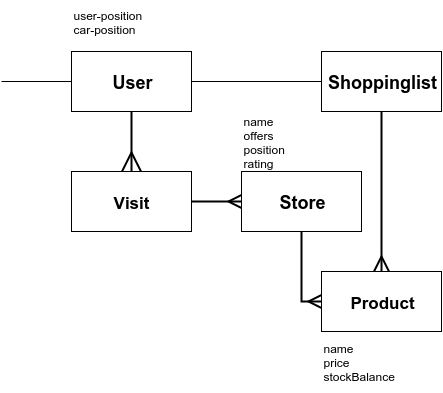
\includegraphics[width=0.7\textwidth]{../files/erdiag.png}
    \caption{Refers to the requirement \textit{Data --- Data relationships}}
    \label{fig:er}
\end{figure}
 
 
 \underline{Data --- Store data} \\ The product shall store data according to figure \ref{fig:store}. 
 
 \begin{figure}[H]
    \centering
    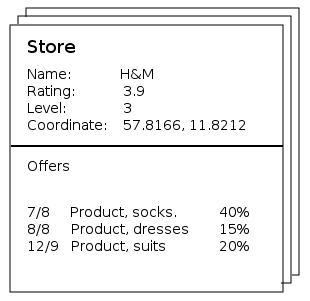
\includegraphics[width=0.4\textwidth]{../files/vw_store.png}
    \caption{Refers to the requirement \textit{Data --- Store data.}}
    \label{fig:store}
\end{figure}
 
\underline{Data --- Product data} \\ The product shall store data according to figure \ref{fig:product}.
 
 \begin{figure}[H]
    \centering
    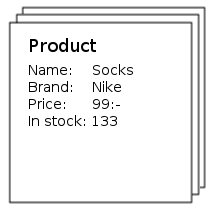
\includegraphics[width=0.35\textwidth]{../files/vw_product.png}
    \caption{Refers to the requirement \textit{Data --- Product data.}}
    \label{fig:product}
\end{figure}
  
 
 %==================================
% Offers
\section{Offer}
Offers are a big part of the product, and the requirements in this section describes how the 
function shall be used to optimize the user-experience in the mall. This is done by restricting 
how often an offer is to be showed and within which ranges stores can notify the user. \\ \par

The product can display offers from any store within 10 meters of the user if the user 
is in the corridor. If the user is in a store, only that store can display an offer. \\�\par

\underline{Offer --- Scenario} \\ The app shall support the following scenario: \\�\par

\textit{
"Jonathan is walking around in the mall with the mall\qu s new application ShopMate installed on his Android phone. He walks past a few stores in the mall 
when he gets a couple of offers from the different stores. Jonathan enters a store he is interested in, and receives an offer specific to that store."
} \\�\par

\underline{Offer --- Receive radius} \\ The product shall display a new offer if the user is within 10 meters to a store.\\ \par

\underline{Offer --- Location offers} \\ The offers shall be relevant to the user\qu s location in the mall.\\ \par
 
\underline{Offer --- Current store} \\ The product shall only display specific offers from the store that the user is currently located in. \\ \par
 
\underline{Offer --- Limit of displaying offers} \\ The product may show a new offer every 120 seconds.

%==================================
% Parking

\section{Parking}
The mall has a great parking lot, and these requirements is stated to aid the users 
when they decide to take their cars to the mall. The two big concerns when it comes 
to parking is the ability to find a free space and later remembering where you parked 
after hours of intense shopping. If these requirements are correctly implemented the users of 
the product shouldn\qu t have to experience these concerns. \\�\par

\underline{Parking --- Scenario} \\ The app shall support the following scenario: \\�\par

\textit{"Jonathan parks his newly renovated Volvo 240 in the parking lot and saves the location of where he parked. 
Jonathan heads to the mall to buy some make-up and comes back later to the parking lot, but has forgotten where he 
parked his car. He uses ShopMate to locate where he parked his car, which guides him to the parking spot."} \\�\par

\underline{Parking --- Register parked car} \\ The user shall be able to register the location of the parked vehicle. \\ \par 

\underline{Parking --- Guide to parked car} \\ The product shall be able to guide the user to their parked vehicle. \\�\par

 \underline{Parking --- Find free parking place} \\ The product shall have the function for displaying what parking places are free. \\�\par

 \underline{Parking --- Guide to free parking place} \\ The product shall have the functionality of assisting the user to a free parking place. 
 
 %==================================
% Transportation
 
\section{Transportation}
This is the section about transportation to the mall using public transport. The product will only provide information on how to get to the mall, not how to get home. \\ \par

\underline{Transportation--- Public transport} \\ The product shall support information about 
departures from the user\qu s current location to the mall, using public transportation.

%==================================
% Smart-watch

\section{Smart-watch}
Below we list requirements that cover the Smart-watch part of the product. The functionality 
that shall be supported by the Smart-watch is not the whole functionality of the product. The 
Smart-watch shall support the following features:

\begin{itemize}
	\item Navigation to any position in the mall including parked car.
	\item Display offers.
	\item Display the customer's shopping list.
\end{itemize} 

\underline{Smart-watch --- General} \\ The product shall support connecting a Smart-watch to it. 
To help the user navigate and get offers from stores without having to interact with their Smartphone. \\ \par 

\underline{Smart-watch --- Navigation} \\ The product shall support navigation on the Smart-watch screen. \\ \par 

\underline{Smart-watch --- Guide to parked car} \\ The product shall support helping the user find where they parked their car. \\ \par 

\underline{Smart-watch --- Offers} \\ The product shall support the functionality to display offers in a Smart-watch. \\ \par 

\underline{Smart-watch --- Shopping list} \\ The product shall be able to display the user\qu s shopping-list on the Smart-watch. \\ \par 

\underline{Smart-watch --- Not required} \\ The product shall work without a Smart-watch. 
Not all customers have Smart-watches and it can therefore not be a requirement to use the product with one. \\�\par

\underline{Smart-watch --- Screen appearance} \\ The Smart-watch screen appearance shall look as in figure \ref{fig:smartwatch}. 

  \begin{figure}[H]
    \centering
    \includegraphics[width=0.5\textwidth]{../files/smartwatches.png}
    \caption{Refers to the requirement \textit{Smart-watch --- Screen appearance.}}
    \label{fig:smartwatch}
\end{figure}

%==================================
% GUI
\section{Graphical User Interface}
Here we list requirements that regard the graphical user interface of the product the product consists of a screen on the 
Smartphone and a screen on the Smart-watch these requirements address both.�\\ \par

 \underline{GUI --- Navigation screen} \\ The product shall provide the screen shown in figure \ref{fig:nav} to help the user navigate.\\�\par 
 
  \begin{figure}[H]
    \centering
    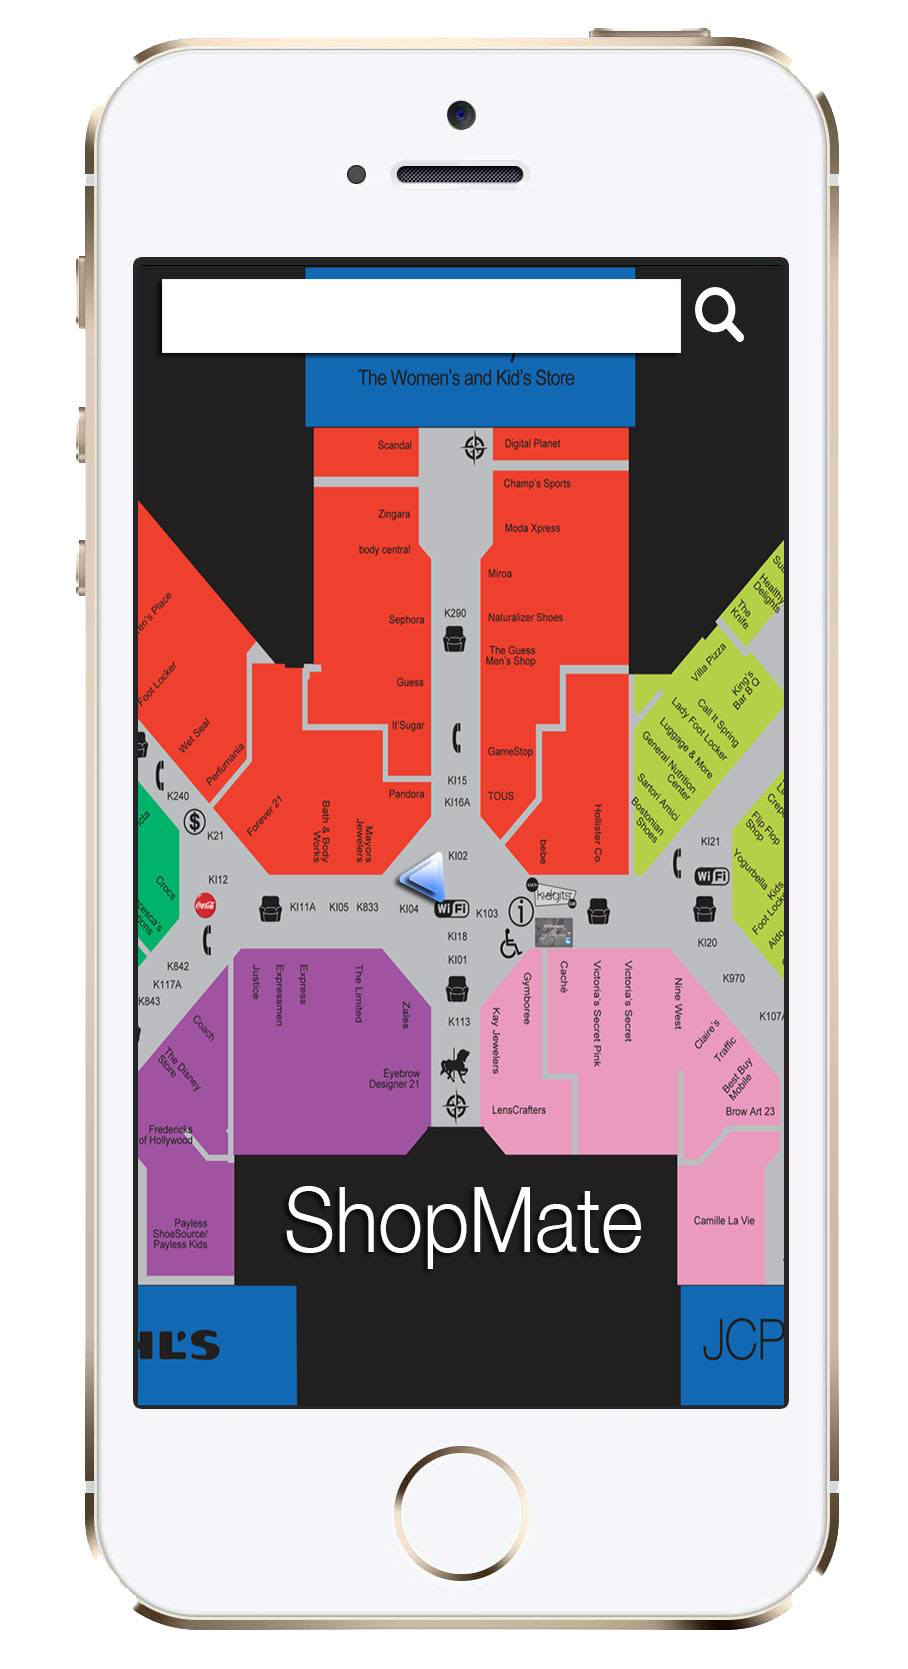
\includegraphics[width=0.3\textwidth]{../files/nav.png}
    \caption{Refers to the requirement \textit{GUI --- Navigation screen.}}
    \label{fig:nav}
\end{figure}

 \underline{GUI --- Understandable interface} \\ The product shall be easy to understand, a novice user shall be able to navigate the interface after the first time the product has been used. \\�\par

\underline{GUI --- Non-covering offers} \\ The product shall show offers from stores without covering the user device screen as seen in figure \ref{fig:noncoveroffer}. \\�\par 

\begin{figure}[H]
    \centering
    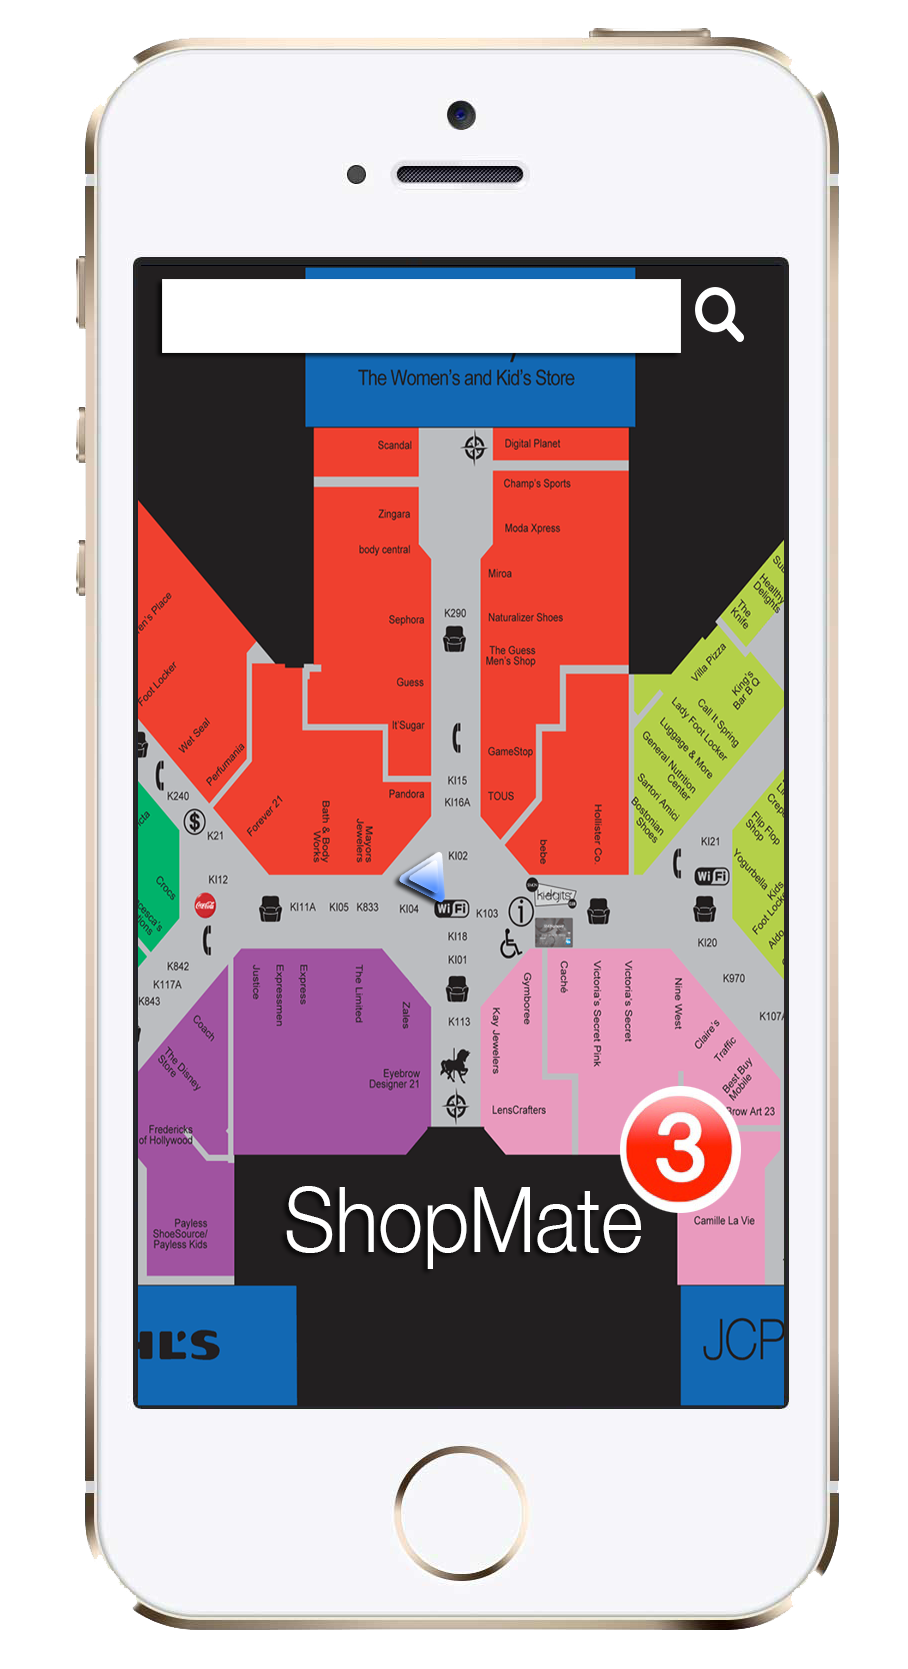
\includegraphics[width=0.3\textwidth]{../files/noncoveroffer.png}
    \caption{Refers to the requirement \textit{GUI --- Non-covering offers}.}
    \label{fig:noncoveroffer}
\end{figure}

\underline{GUI --- Display offers} \\ The product shall be able to enlarge appearing offers and display it as seen in figure \ref{fig:displayoffer}.

\begin{figure}[H]
    \centering
    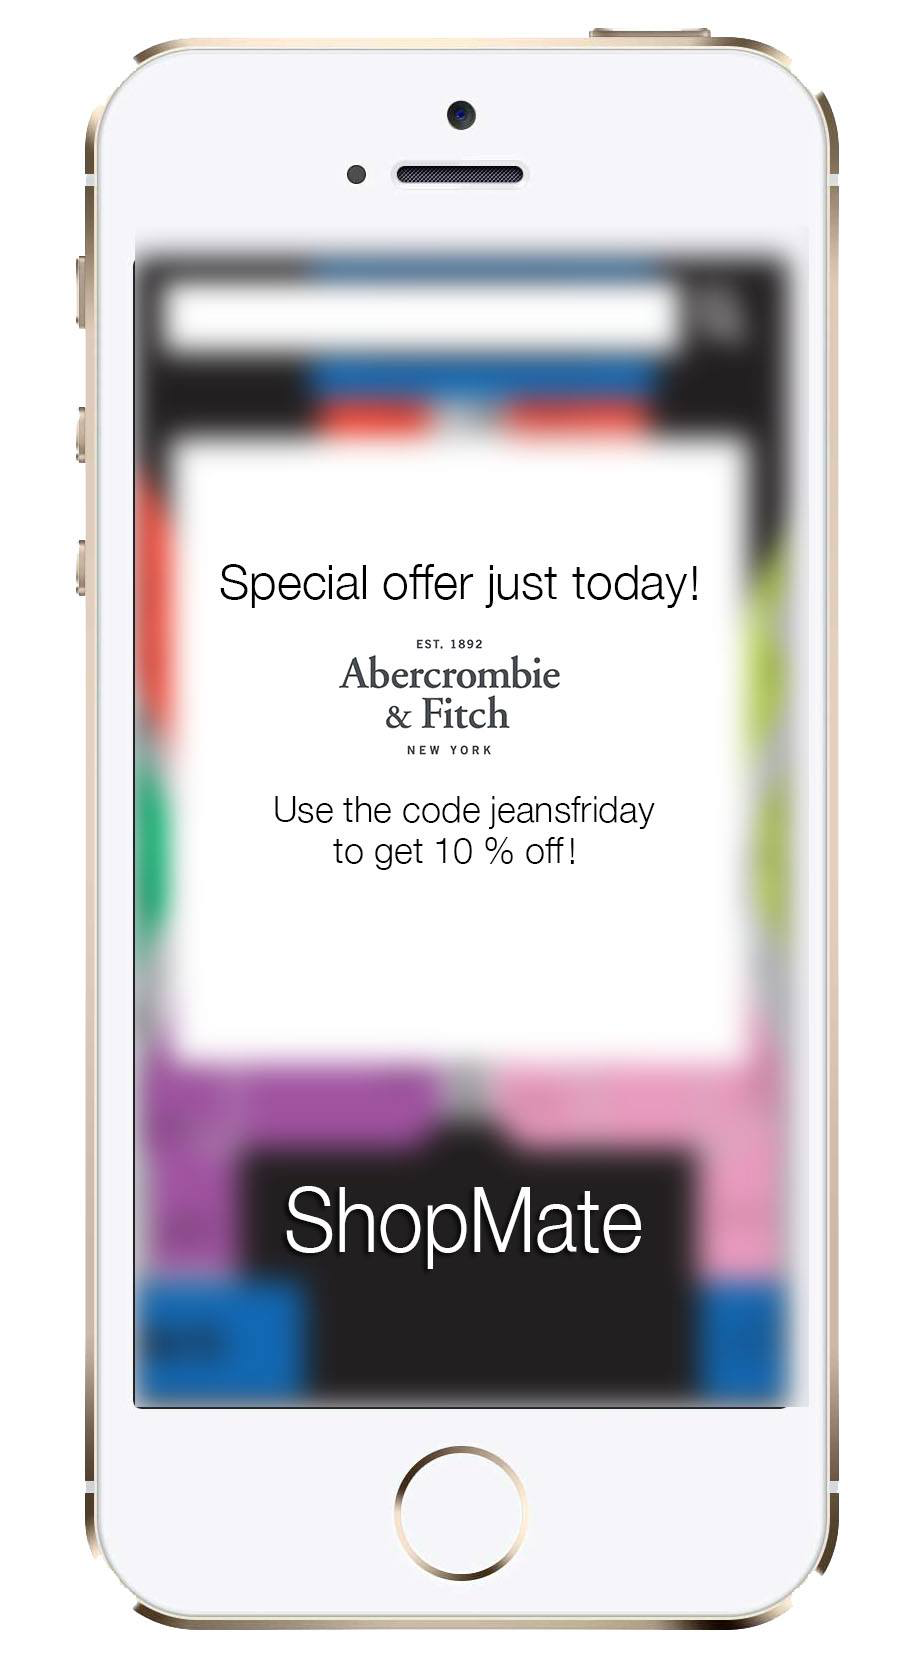
\includegraphics[width=0.3\textwidth]{../files/offer.png}
    \caption{Refers to the requirement \textit{GUI --- Display offers.}}
    \label{fig:displayoffer}
\end{figure}

\underline{GUI --- Register parking spot}�\\  The user shall be able register their parked vehicle as shown in figure \ref{fig:saveparking}.

\begin{figure}[H]
    \centering
    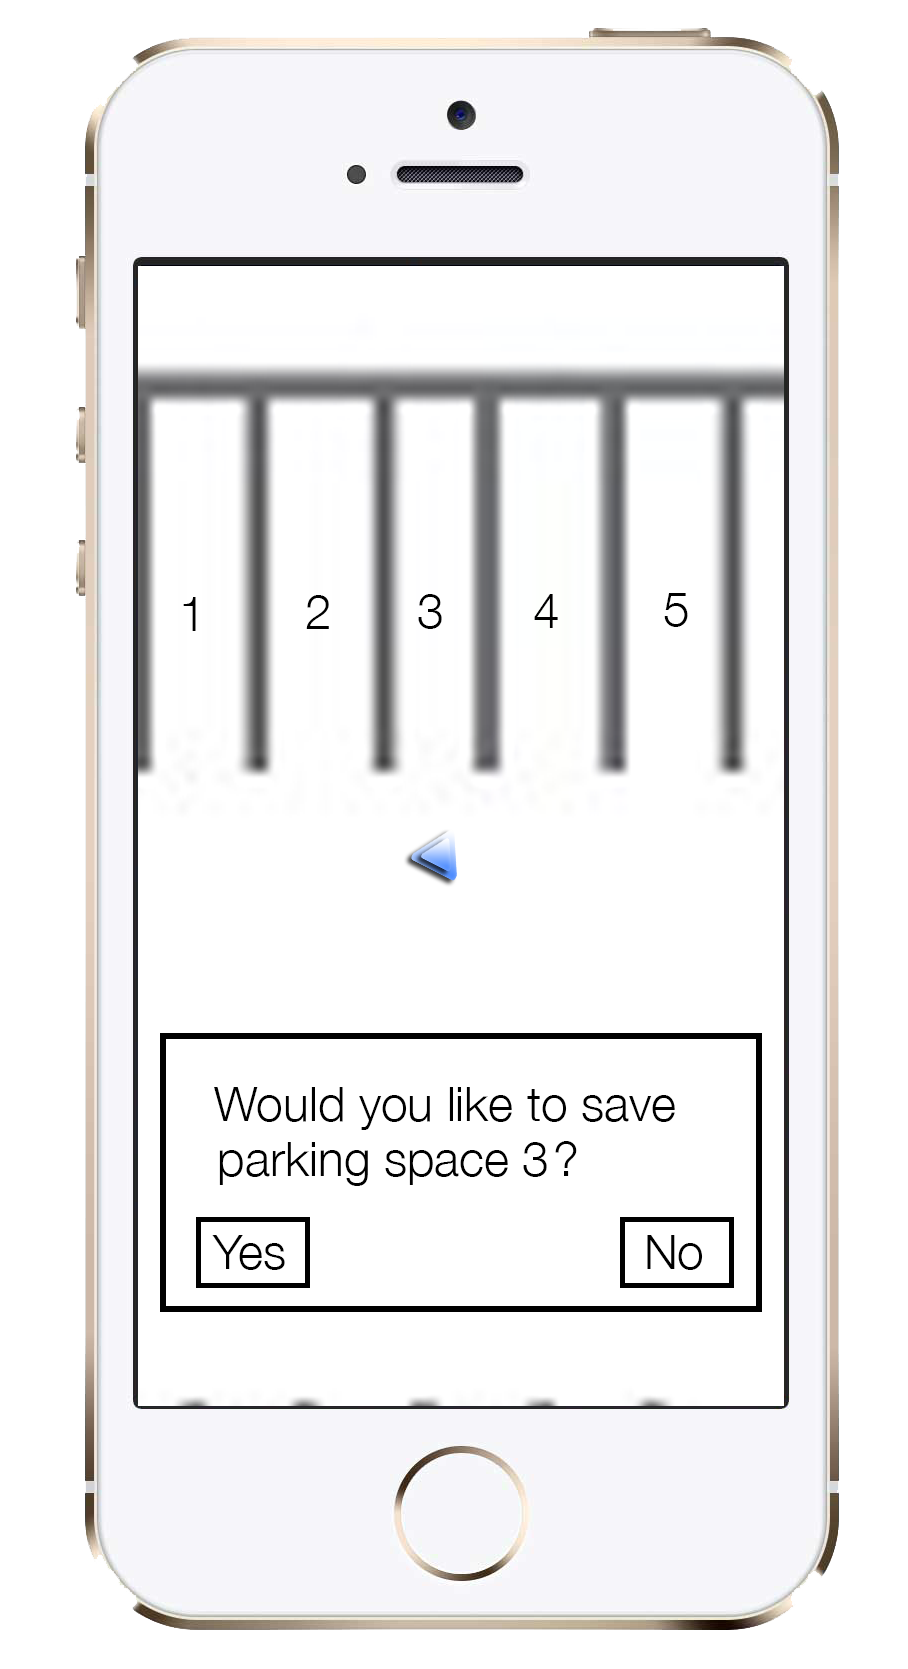
\includegraphics[width=0.3\textwidth]{../files/saveparking.png}
    \caption{Refers to the requirement \textit{GUI --- Register parking spot.}}
    \label{fig:saveparking}
\end{figure}

\underline{GUI --- Navigation to parked vehicle} \\ The product shall be able to navigate a user to their parked vehicle as shown in figure \ref{fig:nav2car}.

\begin{figure}[H]
    \centering
    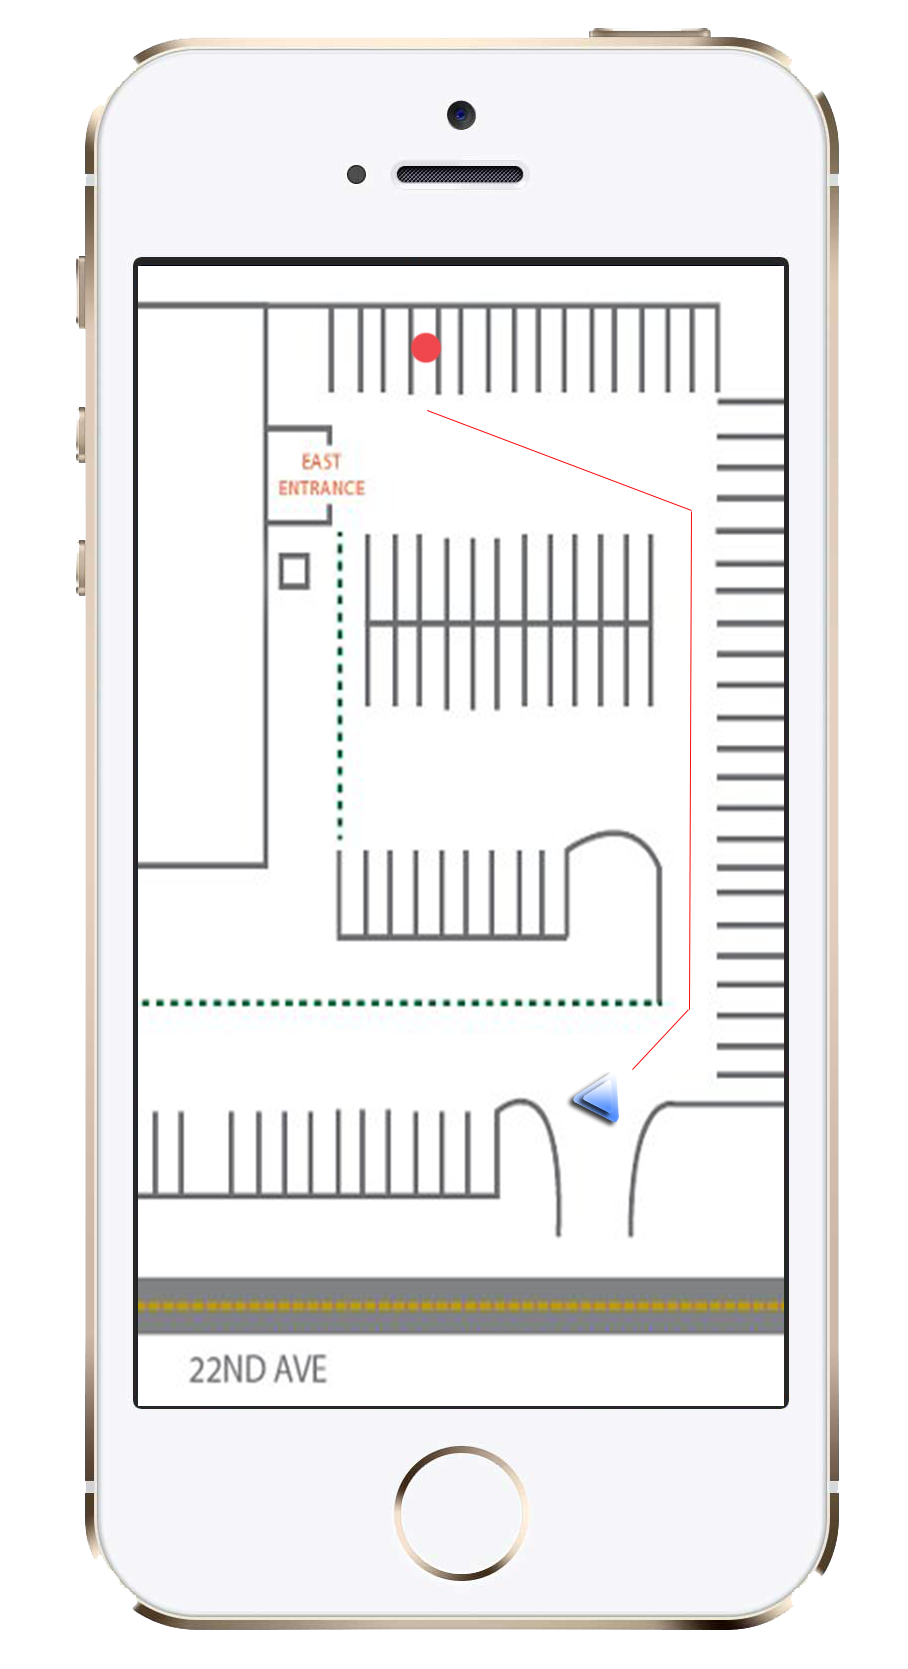
\includegraphics[width=0.3\textwidth]{../files/nav2car.png}
    \caption{Refers to the requirement \textit{GUI --- Display offers.}}
    \label{fig:nav2car}
\end{figure}
 
 %==================================
% Miscellaneous
\section{Miscellaneous}
The requirements listed in this section have no real category. They address 
different types of features and requirements on the product. For example 
when the product does not have internet connection the functionality of the product will be limited. \\�\par


\underline{Misc --- Create shopping list} \\ The user shall be able to create a shopping list in their smartphone. \\ \par 

\underline{Misc --- Store-product info}\\ Searched store-products shall display information about what store has that store-product.�\\�\par

\underline{Misc --- Search by type} \\ The store products shall be searched by type in the user\qu s smartphone. \\�\par

\underline{Misc --- Filter search}\\  The product shall have a function for filtering when searching for products. \\�\par

\underline{Misc --- No connection} \\ The product shall work without being connected to the 
internet, to limit data traffic. Without internet connection the product will help the user navigate 
in the mall and navigate to their parked car using only GPS or any other tracking service. \\�\par

\underline{Misc --- Select store}\\ The user shall be able to select what store and store-product he or she wants to add to the shopping list. \\�\par

\underline{Misc --- Rating system} \\ The product shall have a rating system for stores in the mall that users can use to rate stores. \\�\par

\underline{Misc --- Platform 1} \\ The product shall be implemented for Android devices.\\ \par 
 
 \underline{Misc --- Platform 2} \\ The product shall be implemented for iOS devices. \\�\par
 
 \underline{Misc --- Server up-time} \\ The server shall have at least 99 \% up-time over a year of runtime. \\�\par
  
   \underline{Misc --- Fast server connection} \\ The product shall connect to the server with in 5 seconds after starting the product  95 \% of the time, 
   so the server and the user device is updated with the latest offers and potential new stores. This shall not hinder the application from working. This shall be done in the background.


%===========================
% Appendix
\newpage
\section*{Appendix} \label{app:A} \addcontentsline{toc}{section}{\protect\numberline{}Appendix}

 The appendix contain additional material for this release. 
 
%===========================
% Tables 
 \subsection*{Tables} \addcontentsline{toc}{section}{\protect\numberline{}Tables}
The tables below show which features that are present, depending on what state the user\qu s device have. 

 \begin{table}[h]
\centering
\label{tab:table1}
\resizebox{\textwidth}{!}{%
\begin{tabular}{|c|c|c|c|c|c|c|c|} \hline
                                                                    & \textbf{Feature} & Navigate & Departures to mall & Register parked car & Rate stores & Display offers & Search for store-products \\ \hline
\textbf{Device/state}                                               &                  &          &                    &                     &             &                &                           \\ \hline
\begin{tabular}[c]{@{}c@{}}Smart-watch \\ connected\end{tabular}    &                  & x        &                    &                     &             & x              &                           \\ \hline
\begin{tabular}[c]{@{}c@{}}Smart-watch\\ no connection\end{tabular} &                  & x        &                    &                     &             &                &                           \\ \hline
\begin{tabular}[c]{@{}c@{}}Smartphone\\ connection\end{tabular}     &                  & x        & x                  & x                   & x           & x              & x                         \\ \hline
\begin{tabular}[c]{@{}c@{}}Smartphone\\ no connection\end{tabular}  &                  & x        &                    & x                   &             &                &                        \\  \hline
\end{tabular}
}
\end{table}
 
 % Please add the following required packages to your document preamble:
% \usepackage{graphicx}
\begin{table}[h]
\centering
\label{tab:table2}
\resizebox{\textwidth}{!}{%
\begin{tabular}{|c|c|c|c|c|c|c|} \hline
                                                                    & \textbf{Feature} & Search for products & Info about products & View shopping list & Create shopping list & Info about stores \\ \hline
\textbf{Device/state}                                               &                  &                     &                     &                    &                      &                   \\ \hline
\begin{tabular}[c]{@{}c@{}}Smart-watch \\ connected\end{tabular}    &                  &                    &                     &       x             &                      &                  \\ \hline
\begin{tabular}[c]{@{}c@{}}Smart-watch\\ no connection\end{tabular} &                  &                    &                     &     x               &                      &                   \\ \hline
\begin{tabular}[c]{@{}c@{}}Smartphone\\ connection\end{tabular}     &                  & x                   & x                   & x                  & x                    & x                 \\ \hline
\begin{tabular}[c]{@{}c@{}}Smartphone\\ no connection\end{tabular}  &                  &                    &                     & x                 &                      &                  \\ \hline
\end{tabular}
}
\end{table}
    
\subsection*{Release Plan} \label{app:relplan} \addcontentsline{toc}{subsection}{\protect\numberline{}Release Plan}


%===========================
% R3
\subsubsection*{R3} \addcontentsline{toc}{subsubsection}{\protect\numberline{}R3}

\underline{Team A:}
\begin{tabbing}
Smart-watch --- General~~~~~~~~~~~~~~~~~~~~~~~~~ \= \=  cost: 9 \\
Smart-watch --- Not required \>  \> cost: 2 \\
Navigation - Find user in mall \>  \> cost: 7 \\
GUI --- Understandable interface\>  \>	cost: 3 
\end{tabbing}

\underline{Team B:}
\begin{tabbing}
Parking --- Register parked car~~~~~~~~~~~~~~~~ \= \= cost: 2 \\
Parking --- Find free parking place \>  \>cost: 5 \\
GUI --- Navigation screen \>  \>cost: 4 \\
GUI --- Non covering offers \>  \>cost: 1 
\end{tabbing}

%===========================
% R4
\subsubsection*{R4} \addcontentsline{toc}{subsubsection}{\protect\numberline{}R4}

\underline{Team A:}
\begin{tabbing}
Misc --- Accuracy locate car~~~~~~~~~~~~~~~~~~~~ \= \=cost: 7 \\
Smart-watch --- Navigation \>  \> cost: 4\\
Data --- Database contents \>  \> cost: 8\\
Misc --- Server up-time \>  \> cost: 4\\
Data --- General store information \>  \> cost: 6
\end{tabbing}


\underline{Team B:}
\begin{tabbing}
Smart-watch --- Guide to parked car~~~~~~~~~ \= \=cost: 3 \\
Smart-watch --- Offers \>  \> cost: 3\\
Transportation --- Public transport \>  \> cost: 5\\
Offer --- Location offers \>  \> cost: 4\\
Offer --- Display specific offers \>  \> cost: 3\\
Offer --- Limit of displaying offers \>  \> cost: 2\\
Offer --- Non-annoying commercials \>  \> cost: 6
\end{tabbing}

%===========================
% R5
\subsubsection*{R5} \addcontentsline{toc}{subsubsection}{\protect\numberline{}R5}

\underline{Team A:}
\begin{tabbing}
Smart-watch --- Shopping list~~~~~~~~~~~~~~~~~~ \= \=cost: 3 \\
Navigation - Precision of positioning \>  \> cost: 8\\
Misc - Locate user speed \>  \> cost: 7\\
Misc - Fast server connection \>  \> cost: 8\\
\end{tabbing}

\underline{Team B:}
\begin{tabbing}
Misc --- Create shopping list~~~~~~~~~~~~~~~~~~~ \= \=cost: 4 \\
Misc --- Rating system \>  \> cost: 4 \\
Misc --- Platforms \>  \> cost: 6 
\end{tabbing}

\end{document}